\documentclass[a4paper]{article}
\usepackage[pdftex]{graphicx}
\usepackage[utf8]{inputenc}
\usepackage{enumerate}
\usepackage{siunitx}
\sisetup{locale=DE} 
\usepackage{icomma}
\usepackage{amssymb}
\usepackage{tikz}
\usepackage{href-ul}
\hypersetup{
	colorlinks=true,
	linkcolor=blue,
	urlcolor=blue}
\usepackage{geometry}
\geometry{a4paper, top=15mm, left=15mm, right=15mm, bottom=15mm,
	headsep=10mm, footskip=12mm}

\begin{document}
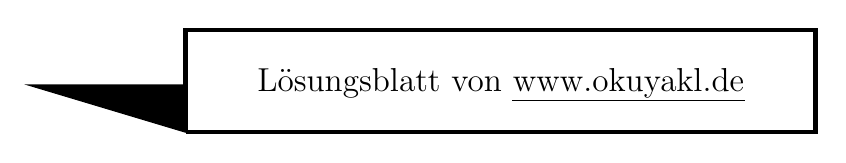
\begin{tikzpicture}(10,3)
	\draw[ultra thick](2,0) --(10,0) -- (10,1.3) --(2,1.3) -- (2,0);
	\draw[fill=black](2,0)-- (0,.6) -- (2,.6) -- (2,0);
	\node at (6,.6) {\large Lösungsblatt von \href{https://www.okuyakl.de}{www.okuyakl.de}};
\end{tikzpicture}
\vspace{0.5 cm}

\noindent {\bf Aufgabe 1. a)}\\
Es sei $M$ die Masse des Phobos, $m$ die Masse des zu beschleunigenden Probekörpers, $G$ die Gravitationskonstante und $R$ der Radius von Phobos. Nach dem Gravitationsgesetz gilt:
$$
\renewcommand{\arraystretch}{2}
\begin{array}{rcll}
m\cdot g_{Ph} & = & { G \cdot M \cdot m \over R^2} & | :m \\
       g_{Ph} & = & { G \cdot M \over R^2} \\
       g_{Ph} & = & { \SI{6,67e-11}{{\meter^3} \over {\kilogram\second^2}} \cdot \SI{1,1e16}{\kilogram} \over (\SI{11000}{\meter})^2} \\
       g_{Ph} & = & \SI{6,1e-3}{\meter \over{ \second^2}}
\end{array}
$$ 
\vspace{0.5 cm}

\noindent {\bf Aufgabe 1. b)}\\
Der Ball soll Phobos auf einer oberflächennahen Kreisbahn umrunden. Hierbei gilt das Kräftegleichgewicht zwischen Zentripetalkraft und Gravitationskraft:
$$
\renewcommand{\arraystretch}{2}
\begin{array}{rcll}
{m\cdot v^2 \over R} & = & { G \cdot M \cdot m \over R^2} & | :m \cdot R\\
v^2 & = & { G \cdot M \over R} & \sqrt{\quad}\\
  v & = & \sqrt{ G \cdot M \over R} \\
  v & = & \sqrt{ \SI{6,67e-11}{{\meter^3} \over {\kilogram\second^2}} \cdot \SI{1,1e16}{\kilogram} \over \SI{11000}{\meter}} \\
  v & = & \SI{8,2}{\meter \over \second}
\end{array}
$$ 
Der Ball soll mit einer Geschwindigkeit von $v=\SI{8,2}{\meter \over \second}$ abgeworfen werden. (Also nicht zu fest werfen, sonst verschwindet er im Weltall!)
\vspace{0.5 cm}

\noindent {\bf Aufgabe 1. c)}\\
Der Umfang der Kreisbahn sei $U = 2 \pi \cdot R$. Dann ist die benötigte Zeit gleich ( zur Erinnerung: $s=v\cdot t$):
$$t = {U \over v}= {2 \pi \cdot R \over v} = {2 \pi \cdot \SI{11000}{\meter} \over \SI{8,2}{\meter \over \second}}= \SI{8430}{\second} \approx \SI{2}{\hour}\SI{20}{\minute}$$
Die Umlaufdauer ist mit über zwei Stunden sehr lang; man sollte sich also etwas zum Lesen mitnehmen...

\vspace{0.5 cm}

\noindent{\bf Aufgabe 2. a)}\\
\begin{itemize}
	\item Größerer Abstand zum Erdmittelpunkt bedeutet geringere Anziehung.
	\item Am  Pol wirkt keine Zentrifugalkraft, diese ist am Äquator maximal.
\end{itemize}
\vspace{0.5 cm}

\noindent{\bf Aufgabe 2. b)}\\
Die Formel zur Berechnung von $g$ lässt sich mit dem Gravitationsgesetz herleiten:
$$
\renewcommand{\arraystretch}{2}
\begin{array}{rcll}
 m g &=& {G \cdot M \cdot m \over r^2} &|:m \\
 g &=& {G \cdot M \over r^2} \\
 g_{Pol} &=& {\SI{6,674e-11}{{\meter^3} \over {\kilogram\second^2}} \cdot\SI{5,972e24}{\kilogram} \over ({\SI{6357e3}{\meter}})^2 }&=\SI{9,860}{\meter \over{ \second^2}}\\
  g_{Aeq}^* &=& {\SI{6,674e-11}{{\meter^3} \over {\kilogram\second^2}} \cdot\SI{5,972e24}{\kilogram} \over ({\SI{6378e3}{\meter}})^2 }&=\SI{9,798}{\meter \over{ \second^2}}\\
\end{array}
$$
$g_{Aeq}^*$ ist noch ohne Berücksichtigung der Zentrifugalbeschleunigung $a_z$; diese muss noch abgezogen werden, um $g_{Aeq}$ zu erhalten:
$$
\renewcommand{\arraystretch}{2}
\begin{array}{rcll}
 a_z &=& {\omega^2 r}\\
     &=& ({2 \pi \over 24 \cdot 60 \cdot \SI{60}{\second}})^2 \cdot  \cdot\SI{6378e3}{\meter}\\
     &=& \SI{5,368e-3}{\meter \over{ \second^2}}
\end{array}
$$
$$g_{Aeq} = g_{Aeq}^* -  a_z = \SI{9,793}{\meter \over{ \second^2}}$$
Hierbei ist zu beachten, dass der Effekt der Fliehkraft viel kleiner ausfällt als der der Radiendifferenz.
Der relative Unterschied der Erdbeschleunigungen ist:
$${g_{Pol}-g_{Aeq}\over g_{Pol}}=0,68\%$$
\vspace{0.5 cm}

\noindent{\bf Aufgabe 3.}\\
Wir setzen Zentrifugal- gleich Gravitationskraft:
$$
\renewcommand{\arraystretch}{2}
\begin{array}{rcll}
{m v^2 \over r} &=& {G  \cdot M \cdot m \over r^2} &|:m v^2 \cdot r^2 \\
r &=& { G \cdot M \over v^2}\\
r &=& {  \SI{6,67e-11}{{\meter^3} \over {\kilogram\second^2}} \cdot 10 \cdot\SI{1,98e30}{\kilogram} \over (\SI{3,0e8}{\meter\over \second})^2} \\
r &=& \SI{15e3}{\meter}
\end{array}
$$
\vspace{0.5 cm}

\noindent{\bf Aufgabe 4.}\\
Die Masse der Erde sei $M_E$, die des Mondes $M_M$.
Der Abstand dieses Punktes zur Erde sei $d-r$. Dann gilt für die Gravitationskräfte:
$$
\renewcommand{\arraystretch}{2}
\begin{array}{rclll}
 F_{G,Erde} &=& F_{G, Mond} \\
{G  \cdot M_E \cdot m \over (d-r)^2} &=& {G  \cdot M_M \cdot m \over r^2} \\
{M_E\over (d-r)^2} &=& { M_M\over r^2} \\
{M_E \over M_M} &=& {(d-r)^2 \over r^2} \\
\sqrt{M_E \over M_M}&=& {d-r \over r} \\
\sqrt{M_E \over M_M}&=& {d\over r}-1 \\
 r &=& { d \over \sqrt{M_E \over M_M}+1} &= {\SI{384400}{\kilo\meter} \over \sqrt {\SI{5,97e24}{\kilogram} \over\SI{7,35e22}{\kilogram}}+1}&=\SI{38400}{\kilo\meter}
\end{array}
$$
\vspace{0.5 cm}

\noindent{\bf Aufgabe 5. a)}\\
Der Radius seiner Umlaufbahn ist:
$$ r = { v \cdot T \over 2 \pi}={\SI{3700}{\meter \over \second} \cdot 130\cdot \SI{60}{\second} \over 2 \pi }=\SI{4,6e6}{\meter}$$
Daraus folgt für den Planetenradius:
$$R=r-\SI{800}{\kilo\meter} = \SI{3,8e6}{\meter} \approx \SI{3800}{\kilo\meter}$$
\vspace{0.5 cm}

\noindent{\bf Aufgabe 5. b)}\\
Wir setzen Gravitation gleich Zentripetalkraft und lösen nach $M$ auf:
$$
\renewcommand{\arraystretch}{2}
\begin{array}{rclll}
{m v^2 \over r} &=& G\cdot {M\cdot m \over r^2} \\
 M &=& {v^2 \cdot r \over G} &= {(\SI{3700}{\meter\over \second})^2 \cdot \SI{3,8e6}{\meter} \over \SI{6,67e-11}{{\meter^3}\over {\kilogram{\second^2}}}} & = \SI{9,4e23}{\kilogram}\\
\end{array}
$$

Damit hat er knapp ein Sechstel der Erdmasse.
\vspace{0.5 cm}

\noindent{\bf Aufgabe 5. c)}\\
Wir setzen Gewichtskraft gleich Gravitation:
$$
\renewcommand{\arraystretch}{2}
\begin{array}{rclll}
mg &=&  G\cdot {M\cdot m \over r^2} \\
 g&=&  G\cdot {M\over r^2} &= \SI{6,67e-11}{{\meter^3} \over {\kilogram\second^2}} \cdot {\SI{9,4e23}{\kilogram} \over (\SI{3,8e6}{\meter})^2 }&=\SI{4,34}{\meter \over {\second^2}}
\end{array}
$$

\begin{center}
	\includegraphics[width=7 cm]{../../viecher/endcomic.pdf}
	
	Hier geht es zurück zum \href{https://www.okuyakl.de/phys/p10kreiL413/aa413.pdf}{Aufgabenblatt}
\end{center}

\end{document}

